\makeatletter\let\ifGm@compatii\relax\makeatother
\documentclass[red]{beamer}

%\usepackage{beamerthemesplit}
\usepackage{listings}
\usepackage{comment}
\usepackage{url}
\usepackage{bm}
\usepackage{tikz}
\usetikzlibrary{arrows.meta}
\usetikzlibrary{shapes.symbols}

\usepackage{hyperref} % has to be last
\hypersetup{
    colorlinks=true,
    linkcolor=blue,
    filecolor=magenta,      
    urlcolor=cyan,
    pdfpagemode=FullScreen,
    }

\tikzset{
    saiarrow/.style={{-Latex}, thick}
}

\newcommand{\isred}[1]{{\color{red} {\bf #1}}} 
\newcommand{\isblue}[1]{{\color{blue}{\bf #1}}} 
\newcommand{\isgreen}[1]{{\color{green} {#1}}} 
\newcommand{\isdarkgreen}[1]{{\color{darkgreen} {#1}}} 
\newcommand{\isorange}[1]{{\color{orange} {#1}}} 

\begin{document}


\setbeamercolor{alerted_text}{fg=cyan}
\xdefinecolor{purplish}{cmyk}{0.75,0.75, 0, 0}
\xdefinecolor{purple}{cmyk}{0.75,0.75, 0, 0}
\colorlet{newred}{red!60!black}

\title{Session 2: Cryptographic operations and security goals}
\author{Slides prepared by UMBC Protocol Analysis Lab}
\date{Last edited \today}
\begin{frame}
\maketitle
\end{frame}

\begin{frame}\frametitle{Symmetric encryption}
\pause
Let \(m\) be a message, \(k\) be a \emph{secret} key, and \(c\) be ciphertext.
\pause
\begin{definition}[Encryption]
A function \(e\) is called an \emph{encryption function} if:
\[
e(m,k) = c
\]
\end{definition}
\pause
\begin{definition}[Decryption]
A function \(d\) is called a \emph{decryption function} if:
\[
d(c,k) = m
\]
\end{definition}
\pause
Common symmetric key algorithms include 3DES, AES, and ChaCha20.
\end{frame}

\begin{frame}\frametitle{Symmetric Encryption Diagram}
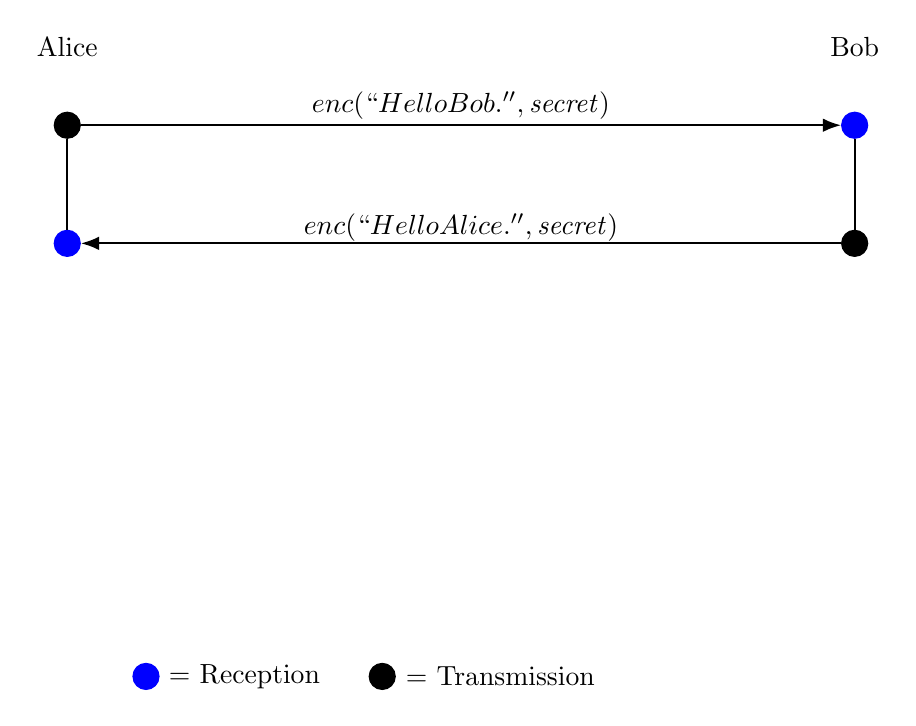
\begin{tikzpicture}
    \node at (0,8) {Alice};
    \node at (10,8) {Bob};
    \node[shape=circle,draw=blue, fill=blue] at (1,0) {};
    \node at (2.25,0) {= Reception};
    \node[shape=circle,draw=black, fill=black] at (4,0) {};
    \node at (5.5,0) {= Transmission};


    \node[shape=circle,draw=black, fill=black] (1) at (0,7) {};
    \node[shape=circle,draw=blue, fill=blue] (2) at (10,7) {};
    \path [saiarrow](1) edge (2);
    
    \node at (5,7.25) {\(enc(\text{``Hello Bob.''}, \mathit{secret})\)};
    
    \node[shape=circle,draw=black, fill=black] (3) at (10,5.5) {};
    \node[shape=circle,draw=blue, fill=blue] (4) at (0,5.5) {};
    
    \path [-,thick](3) edge (2);
    \path [saiarrow](3) edge (4);
    \path [-,thick](1) edge (4);
    
    \node at (5,5.7) {\(enc(\text{``Hello Alice.''},\mathit{secret})\)};
\end{tikzpicture}
\end{frame}

\begin{frame}\frametitle{Asymmetric encryption}
\pause
Let \(m\) be a message, \(pub_k,priv_k\) be a public-private key pair, and \(c\) be ciphertext.
\pause
\begin{definition}[Encryption]
A function \(f\) is \emph{encrypting} if:
\[
f(m,pub_k) = c
\]
\end{definition}
\pause
\begin{definition}[Decryption]
A function \(f\) is \emph{decrypting} if:
\[
f(c,priv_k) = m
\]
\end{definition}
\pause
Common asymmetric key algorithms include RSA, ElGamal, and Elliptic Curve.
\end{frame}

\begin{frame}\frametitle{Asymmetric Encryption Diagram}
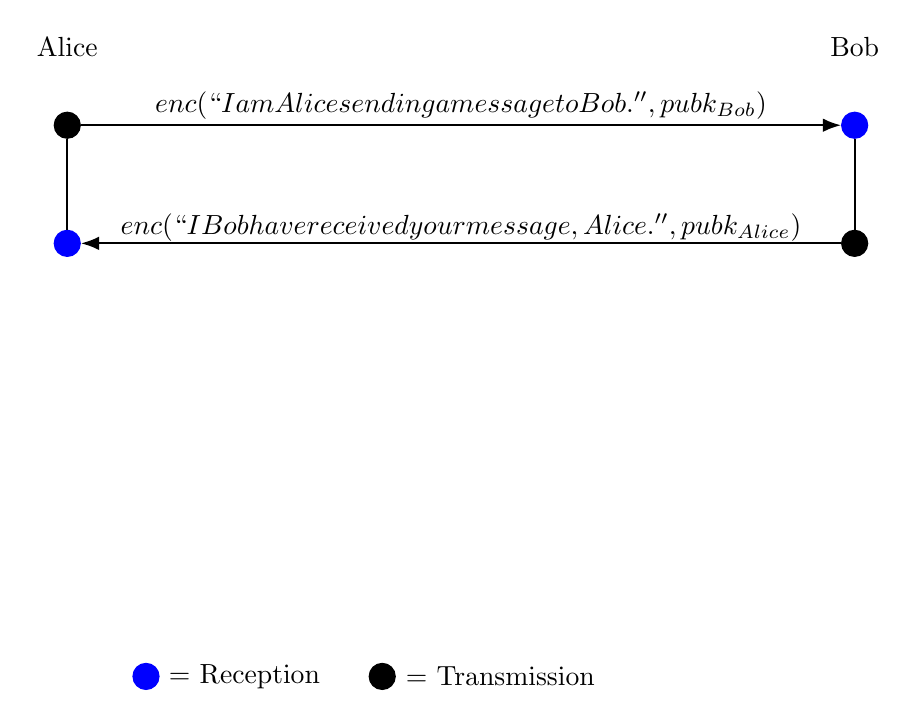
\begin{tikzpicture}
    \node at (0,8) {Alice};
    \node at (10,8) {Bob};
    \node[shape=circle,draw=blue, fill=blue] at (1,0) {};
    \node at (2.25,0) {= Reception};
    \node[shape=circle,draw=black, fill=black] at (4,0) {};
    \node at (5.5,0) {= Transmission};


    \node[shape=circle,draw=black, fill=black] (1) at (0,7) {};
    \node[shape=circle,draw=blue, fill=blue] (2) at (10,7) {};
    \path [saiarrow](1) edge (2);
    
    \node at (5,7.25) {\(enc(\text{``I am Alice sending a message to Bob.''}, pubk_{Bob})\)};
    
    \node[shape=circle,draw=black, fill=black] (3) at (10,5.5) {};
    \node[shape=circle,draw=blue, fill=blue] (4) at (0,5.5) {};
    
    \path [-,thick](3) edge (2);
    \path [saiarrow](3) edge (4);
    \path [-,thick](1) edge (4);
    
    \node at (5,5.7) {\(enc(\text{``I Bob have received your message, Alice.''},pubk_{Alice})\)};
\end{tikzpicture}
\end{frame}

\begin{frame}\frametitle{Signing}
\pause
Let \(m\) be a message, \(pub_k,priv_k\) be a public-private key pair, and \(c\) be ciphertext.
\pause
\begin{definition}[Signing]
A function \(f\) produces a \emph{signature} if:
\[
f(m,priv_k) = c
\]
\end{definition}
\pause
\begin{definition}[Verifying]
A function \(f\) can be used to \emph{verify} if:
\[
f(c,pub_k) = m
\]
\end{definition}
\pause
More or less the same as the asymmetric algorithms.
\end{frame}

\begin{frame}\frametitle{Signing Diagram}
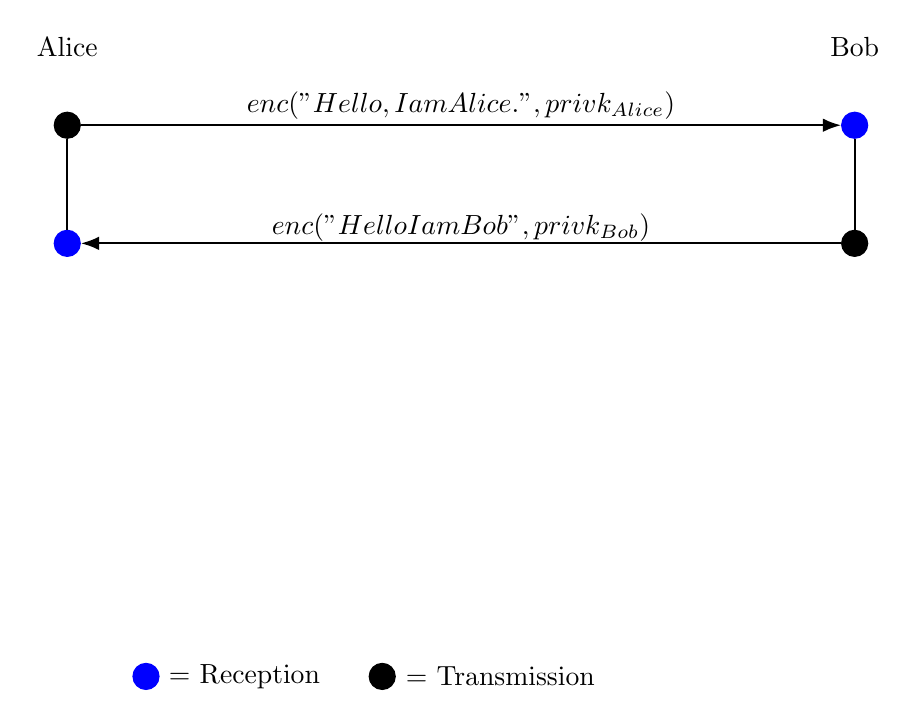
\begin{tikzpicture}
    \node at (0,8) {Alice};
    \node at (10,8) {Bob};
    \node[shape=circle,draw=blue, fill=blue] at (1,0) {};
    \node at (2.25,0) {= Reception};
    \node[shape=circle,draw=black, fill=black] at (4,0) {};
    \node at (5.5,0) {= Transmission};


    \node[shape=circle,draw=black, fill=black] (1) at (0,7) {};
    \node[shape=circle,draw=blue, fill=blue] (2) at (10,7) {};
    \path [saiarrow](1) edge (2);
    
    \node at (5,7.25) {\(enc(\text{"Hello, I am Alice."}, privk_{Alice})\)};
    
    \node[shape=circle,draw=black, fill=black] (3) at (10,5.5) {};
    \node[shape=circle,draw=blue, fill=blue] (4) at (0,5.5) {};
    
    \path [-,thick](3) edge (2);
    \path [saiarrow](3) edge (4);
    \path [-,thick](1) edge (4);
    
    \node at (5,5.7) {\(enc(\text{"Hello I am Bob"},privk_{Bob})\)};
\end{tikzpicture}
\end{frame}

\begin{frame}\frametitle{Hashing}
\pause
Let \(m\) be a message, \(md\) be a message digest.
\pause
\begin{definition}[Hashing]
A function \(h\) is called an \emph{hash function} if:
\begin{enumerate}
\item \(h(m) = md\)
\item It is impractical to determine \(m\) given \(md\).
\item Collision Resistance: It is infeasible to find \(m_1,m_2\) such that \(h(m_1) = h(m_2)\).
\end{enumerate}
\end{definition}
\pause
Common hash functions include the MD family, SHA family, and Skein.
\end{frame}

\begin{frame}\frametitle{Hashing Diagram}
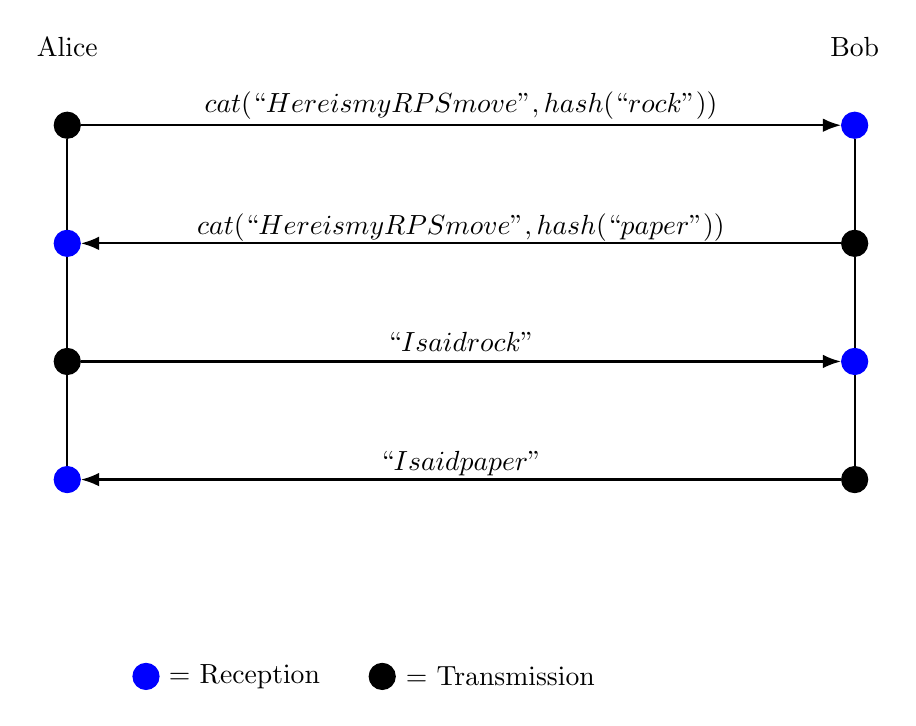
\begin{tikzpicture}
    \node at (0,8) {Alice};
    \node at (10,8) {Bob};
    \node[shape=circle,draw=blue, fill=blue] at (1,0) {};
    \node at (2.25,0) {= Reception};
    \node[shape=circle,draw=black, fill=black] at (4,0) {};
    \node at (5.5,0) {= Transmission};


    \node[shape=circle,draw=black, fill=black] (1) at (0,7) {};
    \node[shape=circle,draw=blue, fill=blue] (2) at (10,7) {};
    \path [saiarrow](1) edge (2);
    
    \node at (5,7.25) {\(cat(\text{``Here is my RPS move"}, hash(\text{``rock"}))\)};
    
    \node[shape=circle,draw=black, fill=black] (3) at (10,5.5) {};
    \node[shape=circle,draw=blue, fill=blue] (4) at (0,5.5) {};
    
    \path [-,thick](3) edge (2);
    \path [saiarrow](3) edge (4);
    \path [-,thick](1) edge (4);
    
    \node at (5,5.7) {\(cat(\text{``Here is my RPS move"}, hash(\text{``paper"}))\)};

    \node[shape=circle,draw=black, fill=black] (5) at (0,4) {};
    \node[shape=circle,draw=blue, fill=blue] (6) at (10,4) {};
    \path [saiarrow](5) edge (6);

    \path [-,thick](3) edge (6);
    \path [-,thick](4) edge (5);
    
    \node at (5,4.25) {\(\text{``I said rock"}\)};
    
    \node[shape=circle,draw=black, fill=black] (7) at (10,2.5) {};
    \node[shape=circle,draw=blue, fill=blue] (8) at (0,2.5) {};
    
    \path [-,thick](7) edge (6);
    \path [saiarrow](7) edge (8);
    \path [-,thick](5) edge (8);
    
    \node at (5,2.7) {\(\text{``I said paper"}\)};
\end{tikzpicture}
\end{frame}

\title{Security Goals}
\author{How do we know a protocol is secure?}
\date{}
\begin{frame}
\maketitle
\end{frame}

\begin{frame}\frametitle{What is a security goal?}
\pause
A \emph{security goal} is a goal that we assign for a given protocol to evaluate if it is sufficiently secure for application.

\pause
Security goals formalize our notion of ``secure''.

\bigskip
\pause
Not every protocol has the same requirement for security.

\pause
\textbf{Air-gapped case:}
\pause
Since there is no one else on the network, we can send the information in plaintext.

\pause
\textbf{Home network:}
\pause
The adversary is not observing every single packet, but may be able to observe snippets.

\pause
\textbf{Coffee shop:}
\pause
A lot of people on the network, so we need a very secure protocol.
\end{frame}

\begin{frame}\frametitle{Common security goals}
\pause
\textbf{Confidentiality:} In a two-party communication protocol, confidentiality holds if no third party is able to access the information sent.

\pause
\textbf{Agreement:} In a two-party communication protocol, agreement holds if both parties agree on some set of data values in the protocol.
These values are then used to derive the key.

\pause
What security goals might we need for the air-gapped, home, and coffee shop networks?
\end{frame}

\begin{frame}\frametitle{Other common security goals}
\begin{enumerate}
\item Aliveness
\pause
\item Weak Agreement
\pause 
\item Non-injective Agreement
\pause
\item A specific relay party cannot read the message
\pause
\item The message must be timestamped
\pause
\item Perfect forward secrecy
\pause
\item Crypto primitives are resistant to a predefined attack
\end{enumerate}
\end{frame}


\title{Needham Schroeder}
\author{Designing a meeting protocol, and beyond}
\date{}
\begin{frame}
\maketitle
\end{frame}

\begin{frame}\frametitle{Strand spaces}
A \emph{strand space} is a formalism used to determine the security of a network protocol
\begin{itemize}
\item Fábrega, F. J. T., Herzog, J. C., \& Guttman, J. D. (1998, May). \href{https://www.mitre.org/sites/default/files/pdf/guttman_strands.pdf}{Strand spaces: Why is a security protocol correct?}
\item Represent honest communicants and intruders as ``strands''
\item Parallel / sequential composability.
\end{itemize}
\end{frame}

\begin{frame}\frametitle{Example of a strand}
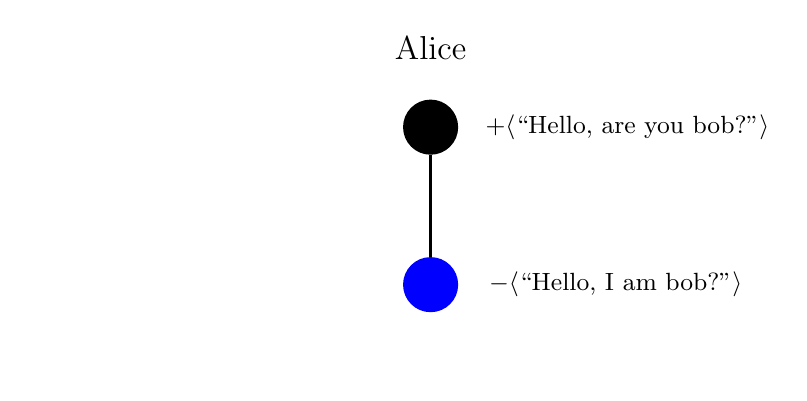
\begin{tikzpicture}[
    node distance=2cm,
    every node/.style={font=\small},
    dot/.style={circle, minimum size=0.7cm, inner sep=0pt},
    arrow/.style={-{Latex[length=4mm]}, very thick}
]

    \node at (0,0) {};
    \node at (5,4) {\large Alice};
    \pause
    \node at (7.5,3) {\(+\langle\)``Hello, are you bob?''\(\rangle\)};
    \node[dot, fill=black] (A1) at (5,3) {};
    \pause
    \node[dot, fill=blue] (A2) at (5,1) {};
    \node at (7.35,1) {\(-\langle\)``Hello, I am bob?''\(\rangle\)};
    \draw[very thick] (A1) -- (A2);
\end{tikzpicture}
\end{frame}

\begin{frame}\frametitle{Strand space}
\hspace{-2.2em}
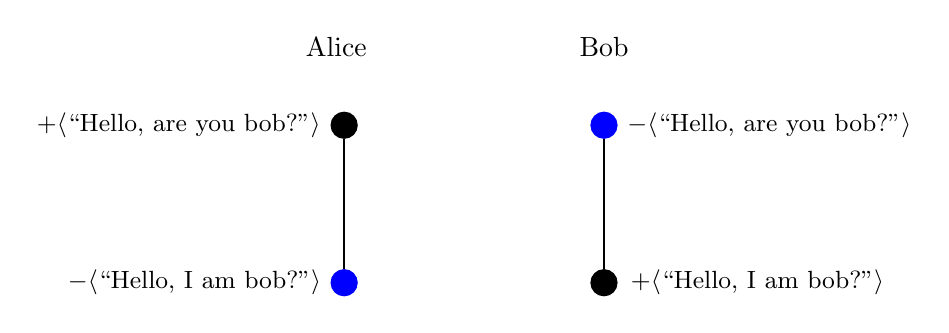
\begin{tikzpicture}
    \node at (2,8) {Alice};
    \node at (0,7) {\small\(+\langle\)``Hello, are you bob?''\(\rangle\)};    \node[shape=circle,draw=blue, fill=blue] (1) at (2.1,5) {};
    \node at (0.2,5) {\small\(-\langle\)``Hello, I am bob?''\(\rangle\)};
    \node[shape=circle,draw=black, fill=black] (4) at (2.1,7) {};

    \node at (5.4,8) {Bob};
    \node at (7.5,7) {\small \(-\langle\)``Hello, are you bob?''\(\rangle\)};
    \node[shape=circle,draw=black, fill=black] (2) at (5.4,5) {};
    \node at (7.35,5) {\small \(+\langle\)``Hello, I am bob?''\(\rangle\)};
    \node[shape=circle,draw=blue, fill=blue] (3) at (5.4,7) {};

    \path [-,thick](3) edge (2);
    \path [-,thick](1) edge (4);
\end{tikzpicture}
\end{frame}

\begin{frame}\frametitle{A completed protocol?}
\hspace{-2.2em}
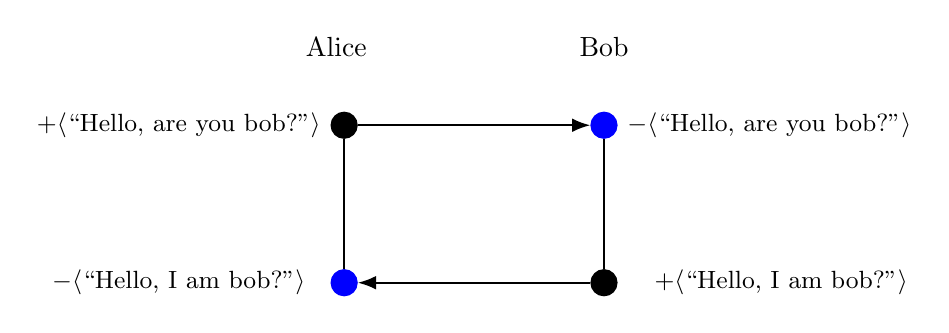
\begin{tikzpicture}
    \node at (2,8) {Alice};
    \node at (0,7) {\small\(+\langle\)``Hello, are you bob?''\(\rangle\)};    \node[shape=circle,draw=blue, fill=blue] (1) at (2.1,5) {};
    \node at (0,5) {\small\(-\langle\)``Hello, I am bob?''\(\rangle\)};
    \node[shape=circle,draw=black, fill=black] (4) at (2.1,7) {};

    \node at (5.4,8) {Bob};
    \node at (7.5,7) {\small \(-\langle\)``Hello, are you bob?''\(\rangle\)};
    \node[shape=circle,draw=black, fill=black] (2) at (5.4,5) {};
    \node at (7.65,5) {\small \(+\langle\)``Hello, I am bob?''\(\rangle\)};
    \node[shape=circle,draw=blue, fill=blue] (3) at (5.4,7) {};

    \path [-,thick](3) edge (2);
    \path [saiarrow](2) edge (1);
    \path [-,thick](1) edge (4);
    \path [saiarrow](4) edge (3);
\end{tikzpicture}
\end{frame}

\begin{frame}\frametitle{Strands can lie}
\hspace{-2.2em}
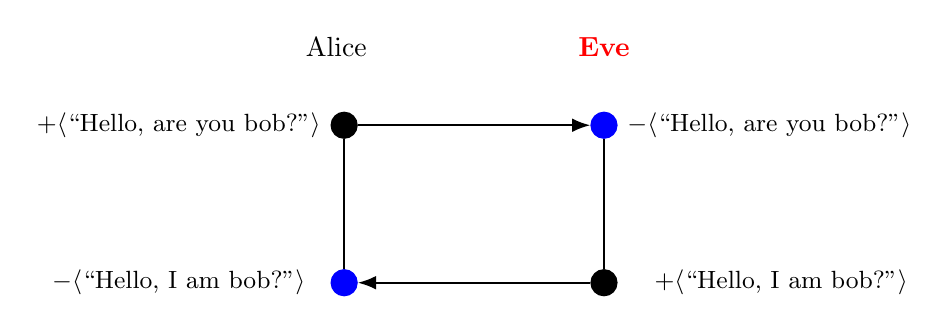
\begin{tikzpicture}
    \node at (2,8) {Alice};
    \node at (0,7) {\small\(+\langle\)``Hello, are you bob?''\(\rangle\)};    \node[shape=circle,draw=blue, fill=blue] (1) at (2.1,5) {};
    \node at (0,5) {\small\(-\langle\)``Hello, I am bob?''\(\rangle\)};
    \node[shape=circle,draw=black, fill=black] (4) at (2.1,7) {};

    \node at (5.4,8) {\isred{Eve}};
    \node at (7.5,7) {\small \(-\langle\)``Hello, are you bob?''\(\rangle\)};
    \node[shape=circle,draw=black, fill=black] (2) at (5.4,5) {};
    \node at (7.65,5) {\small \(+\langle\)``Hello, I am bob?''\(\rangle\)};
    \node[shape=circle,draw=blue, fill=blue] (3) at (5.4,7) {};

    \path [-,thick](3) edge (2);
    \path [saiarrow](2) edge (1);
    \path [-,thick](1) edge (4);
    \path [saiarrow](4) edge (3);
\end{tikzpicture}
\end{frame}

\begin{frame}\frametitle{Needham Schroeder}
\begin{tikzpicture}
    \node at (0,8) {Alice};
    \node at (10,8) {Bob};
    \node[shape=circle,draw=blue, fill=blue] at (1,0) {};
    \node at (2.25,0) {= Reception};
    \node[shape=circle,draw=black, fill=black] at (4,0) {};
    \node at (5.5,0) {= Transmission};

    \pause
    \node[shape=circle,draw=black, fill=black] (1) at (0,7) {};
    \node[shape=circle,draw=blue, fill=blue] (2) at (10,7) {};
    \path [saiarrow](1) edge (2);
    
    \node at (5,7.25) {\(enc(N_a, Alice, pubk_{Bob})\)};

    \pause
    \only<3> {\node (nonceA) at (5,5) {\fbox{\textbf{nonce:} a \emph{fresh}, cryptographic random number generated by Alice.}}};
    \only<3> {\node[shape=circle, draw=black, minimum size=1.5em, thick] (circA) at (4.07,7.25) {}};
    \only<3> {\draw (circA) -- (nonceA)};
    
    \pause
    \node[shape=circle,draw=black, fill=black] (3) at (10,5.5) {};
    \node[shape=circle,draw=blue, fill=blue] (4) at (0,5.5) {};
    
    \path [-,thick](3) edge (2);
    \path [saiarrow](3) edge (4);
    \path [-,thick](1) edge (4);
    
    \node at (5,5.7) {\(enc(N_a,N_b,pubk_{Alice})\)};

    \pause   
    \only<5> {\node (nonceB) at (5,4) {\fbox{\textbf{nonce:} a \emph{fresh}, cryptographic random number generated by Bob.}}};
    \only<5> {\node[shape=circle, draw=black, minimum size=1.5em, thick] (circB) at (4.82,5.73) {}};
    \only<5> {\draw (circB) -- (nonceB)};

    \pause
    \node[shape=circle,draw=blue, fill=black] (5) at (0,4) {};
    \node[shape=circle,draw=blue, fill=blue] (6) at (10,4) {};
    
    \path [-,thick](6) edge (3);
    \path [saiarrow](5) edge (6);
    \path [-,thick](5) edge (4);
    
    \node at (5,4.2) {\(enc(N_b,pubk_{Bob})\)};

    \pause
    \node at (5,2) {Is this protocol secure against the Dolev-Yao Adversary?};
    
\end{tikzpicture}
\end{frame}

\begin{frame}\frametitle{Cryptographic Protocol Shapes Analyzer}
\begin{itemize}
\item Tool for analyzing and developing secure protocols.
\item Enumerates all possible executions of a protocol.
\item Assumes a Dolev-Yao adversary.
\item Developed by MITRE, available at: \url{https://github.com/mitre/cpsa}
\end{itemize}
\end{frame}

\begin{frame}\frametitle{Analyze Needham-Schroeder}
Define protocol \emph{roles} and \emph{skeletons}.

Run CPSA to produce \emph{shapes}.

Analyze \emph{shapes} for expected and unexpected behavior.
\end{frame}

\begin{frame}\frametitle{Needham Schroeder Attack}
\pause
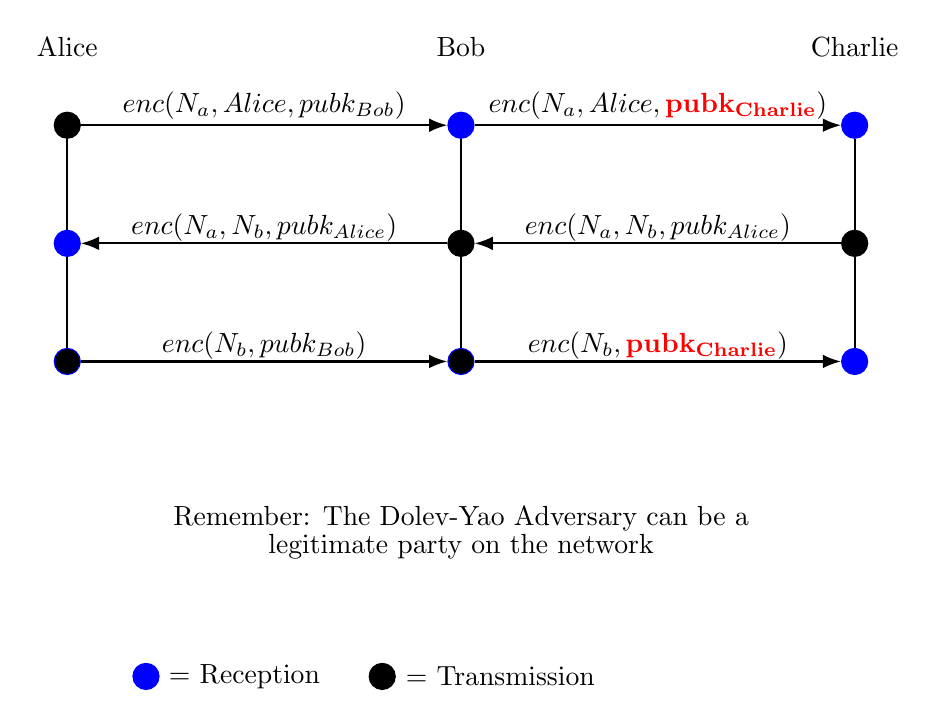
\begin{tikzpicture}
    \node at (0,8) {Alice};
    \node at (10,8) {Charlie};
    \node at (5,8) {Bob};
    \node[shape=circle,draw=blue, fill=blue] at (1,0) {};
    \node at (2.25,0) {= Reception};
    \node[shape=circle,draw=black, fill=black] at (4,0) {};
    \node at (5.5,0) {= Transmission};

    \node[shape=circle,draw=black, fill=black] (1) at (0,7) {};
    \node[shape=circle,draw=blue, fill=blue] (2) at (10,7) {};
    \node[shape=circle,draw=blue, fill=blue] (1m) at (5,7) {};
    
    \path [saiarrow](1) edge (1m);
    \path [saiarrow](1m) edge (2);
    
    \node at (2.5,7.25) {\(enc(N_a, Alice, pubk_{Bob})\)};
    \node at (7.5,7.25) {\(enc(N_a, Alice, \isred{pubk_{Charlie}})\)};
    
    \node[shape=circle,draw=black, fill=black] (3) at (10,5.5) {};
    \node[shape=circle,draw=blue, fill=blue] (4) at (0,5.5) {};
    \node[shape=circle,draw=black, fill=black] (3m) at (5,5.5) {};
    
    \path [-,thick](3) edge (2);
    \path [saiarrow](3) edge (3m);
    \path [saiarrow](3m) edge (4);
    \path [-,thick](1) edge (4);
    \path [-,thick](1m) edge (3m);
    
    \node at (7.5,5.7) {\(enc(N_a,N_b,pubk_{Alice})\)};
    \node at (2.5,5.7) {\(enc(N_a,N_b,pubk_{Alice})\)};

    \node[shape=circle,draw=blue, fill=black] (5) at (0,4) {};
    \node[shape=circle,draw=blue, fill=blue] (6) at (10,4) {};
    \node[shape=circle,draw=blue, fill=black] (5m) at (5,4) {};
    
    \path [-,thick](6) edge (3);
    \path [saiarrow](5) edge (5m);
    \path [saiarrow](5m) edge (6);
    \path [-,thick](5) edge (4);
    \path [-,thick](3m) edge (5m);
    
    \node at (2.5,4.2) {\(enc(N_b,pubk_{Bob})\)};
    \node at (7.5,4.2) {\(enc(N_b,\isred{pubk_{Charlie}})\)};

    \node at (5,2) {Remember: The Dolev-Yao Adversary can be a };
    \node at (5,1.65) {legitimate party on the network};
    
\end{tikzpicture}
\end{frame}

\begin{frame}\frametitle{Homework}
\begin{center}
{\Huge Fix your protocol}
\end{center}
\pause
Last time, you created a meeting protocol.

Do you think your meeting protocol withstands the Dolev-Yao adversary?

\pause
Model your protocol in CPSA and see if there is an attack!

See if you can fix your protocol so that there is no more attack.
\end{frame}

\begin{frame}\frametitle{Survey}
Fill in details about the survey here!
\end{frame}

\end{document}